%% =============================================================================
%% Mathematische Grundlagen - Grundbegriffe
%% Kapitel 04 - Mengen
%% Autor: Andreas Zeh-Marschke
%% Datum: 2025-04-09
%% =============================================================================

\chapter{Naive Mengenlehre}
\label{cha:Gdl-K04-Mengen}

%% -----------------------------------------------------------------------------
%\begin{unit}
In diesem Kapitel werden die wichtigsten Grundbegriffe und Notationen der 
Mengenlehre eingeführt. Begriffe und Symbolik der Mengenlehre und der formalen 
Logik gestatten zusammen eine präzise Formulierung mathematischer Aussagen.

Zuerst werden \textbf{Mengen} eingeführt (Abschnitt \ref{sec:Mengen:Mengen}), 
bevor dann \textbf{Teilmengen} und die \textbf{Potenzmenge} definiert werden
(Abschnitt \ref{sec:Mengen:Teilmengen und Potenzmenge}). Im Abschnitt 
\ref{sec:Mengen:Operationen von Mengen} werden \textbf{Operationen von Mengen} 
betrachtet und die Mengenarithmetik untersucht. Im anschließenden Abschnitt
\ref{sec:Mengen:Klasseneinteilung} werden \textbf{Klasseneinteilungen}, das 
heißt Zerlegungen von Mengen, betrachtet, die eine Verbindung zu
Äquivalenzrelationen haben, die erst im nächsten Kapitel betrachtet werden,
beschrieben. Ein wichtiges Beispiel von Mengen, die ebenfalls im nachfolgenden
Kapitel eine weiter gehende Bedeutung haben, ist das 
\textbf{kartesische Produkt}, welches im abschließenden Abschnitt
\ref{sec:Mengen:Kartesisches Produkt} definiert wird.
%\end{unit}

%%------------------------------------------------------------------------------
%% Abschnitt: Mengen
%%------------------------------------------------------------------------------
\section{Mengen}
\label{sec:Mengen:Mengen}

%% --- Definition und Beschreibung ---------------------------------------------
%\subsection*{Definition und Beschreibung}

%% -----------------------------------------------------------------------------
\begin{Unit}[Definition][Menge]
Die grundlegende Definition einer Menge geht zurück auf Georg Cantor
\footnote{Georg Cantor (1845-1918) deutscher Mathematiker
\url{https://de.wikipedia.org/wiki/Georg_Cantor}}.

\begin{Definition}
Eine \Begriff{Menge} ist die Zusammenfassung bestimmter, 
wohlunterschiedener Objekte unserer Anschauung oder unseres Denkens zu einem 
Ganzen. Die Objekte, die zu einer Menge zusammengefasst werden heißen 
\Begriff{Elemente} der Menge. \\
Ist $M$ eine Menge und $x$ ein Objekt, so wird $x \in M$ geschrieben, wenn 
$x$ ein Element von $M$ ist und $x \notin M$, wenn $x$ nicht Element von 
$M$ ist.
\end{Definition}

Mengen können entweder durch die Aufzählung ihrer Elemente oder die Angabe der 
Eigenschaften der Elemente der Menge beschrieben werden. Die Elemente werden in 
geschweifter Klammer geschrieben.
\end{Unit}
\Translation{Menge}{set}
\Translation{Element}{element}

%% -----------------------------------------------------------------------------
\begin{Unit}[Beispiel]
Einige Beispiele von Beschreibungen von Mengen:
\begin{enumerate}
\item
  $A$ sei die Menge aller Farben einer Verkehrsampel. \\
  $A$ := \{rot, gelb, grün\}
\item
  $B$ sei die Menge aller möglichen Farbzustände einer Verkehrsampel. \\
  $B$ := \{rot, rot-gelb, grün, gelb, gelb-blinkend, aus\}
\item
  $C$ sei die Menge aller geraden Zahlen.
\item  
  $D$ sei die Menge aller Quadratzahlen kleiner als 100. \\
  $D$ := \{1, 4, 9, 16, 25, 36, 49, 64, 81\}
\item  
  $E$ sei die Menge der Studentinnen und Studenten einer Vorlesung.
\end{enumerate}
\end{Unit}

%% -----------------------------------------------------------------------------
\begin{Unit}[Beispiel]
Die Beschreibung von Mengen kann auch mit Hilfe von Prädikaten erfolgen.

\begin{enumerate}
\item
  Es sei $P_3$ das Prädikat \enquote{ist gerade}, also $P_3(x)$ die 
  Aussageform \enquote{x ist gerade}. Weiter sei 
  $C\ :=\ \{ x \mid P_3(x) \}$ die Menge, deren Elemente diejenigen Objekte 
  sind, für welche die Aussage $P_3(x)$ wahr   ist.
\item
  Es seien $P_4$ das Prädikat \enquote{ist Quadratzahl} und $P_4(x)$ die 
  Aussageform \enquote{x ist Quadratzahl}. Weiter seien $Q_4$ das Prädikat
  \enquote{ist kleiner als 100} und $Q_4(x)$ die Aussageform \enquote{x ist 
  kleiner als 100}. Die Menge der Quadratzahlen kleiner als 100 kann durch
  $D := \{ x \mid P_4(x) \land Q_4(x) \}$ beschrieben werden.
\end{enumerate}
\end{Unit}

%% -----------------------------------------------------------------------------
\begin{Unit}[Anmerkung]
Die obige Definition der Menge kann zu Widersprüchen führen. Die Bildung der 
\enquote{Menge} $M$ aller Mengen $X$, die nicht Element von sich selbst sind, 
führt zu einem Widerspruch. Gehört $M$ selbst zu dieser Menge oder nicht? Dies
ist unter dem Namen \emph{Antinomie von Russell} bekannt, benannt nach dem
Bertrand Russell\footnote{Bertrand Russell (1872-1970) britischen 
Mathematiker und Philosoph , Nobelpreis für Literatur 1950)}
\index[names]{Russell, Bertrand}. Diese Problematik wird hier nicht weiter 
verfolgt. Daher wird hier nur die sogenannten \enquote{naiven} Mengenlehre
betrachtet.
\end{Unit}

%% --- Wichtige Mengen ---------------------------------------------------------
%\subsection*{Wichtige Mengen}

%% -----------------------------------------------------------------------------
\begin{Unit}[Beispiel - Wichtige grundlegende Mengen]
Beispiele wichtiger Mengen aus der Mathematik:
\begin{enumerate}
\item Menge der \textbf{natürlichen Zahlen}\footnote{Die 0 zählt hier
  \textbf{nicht}\index{natürliche Zahl} zu den natürlichen Zahlen!}: \\
  $\NN = \{ n \mid n\text{ ist natürliche Zahl} \} = \{ 1, 2, 3, \ldots \} $
  
\item Menge der natürlichen Zahlen mit der $0$: \\
  $\NN_0 = \{ n \mid n\text{ ist natürliche Zahl oder }0 \}
  = \{ 0, 1, 2, \ldots \}  $
  
\item Menge der \Begriff{Primzahl}en: \\
  $\PP = \{ p \mid p\text{ ist Primzahl} \} 
    =\{p \mid p\ ist\ Primzahl\} 
            = \{ 2, 3, 5, 7, 11, \ldots \} $

\item Menge der \textbf{ganzen Zahlen}\index{ganze Zahl}: \\
  $\ZZ = \{z \mid z\text{ ist ganze Zahl}\} 
            = \{ 0, \pm 1, \pm 2, \pm 3, \ldots \} $

\item Menge der \textbf{rationalen Zahlen}\index{rationale Zahl}: \\
  $\QQ = \{ x \mid x\text{ ist rationale Zahl}\}
            = \{ x = \frac{p}{q} \mid p \in \ZZ\ und\ q \in \NN \} $

\item Menge der \textbf{reellen Zahlen}\index{reelle Zahl}: \\
  $\RR = \{ x \mid x\text{ ist reelle Zahl} \} $
\end{enumerate}
\end{Unit}
\Translation{natürliche Zahl}{natural number}
\Translation{Primzahle}{prime number}
\Translation{ganze Zahl}{integer}
\Translation{rationale Zahl}{rational number}
\Translation{reelle Zahl}{real number}

%% -----------------------------------------------------------------------------
\begin{Unit}[Beispiel]
Für die nachfolgenden Beispiel sei stets die Grundmenge $X$ einer der Mengen
$\ZZ$, $\QQ$ oder $\RR$.

\begin{enumerate}
  \item Menge der positiven Zahlen: \\
    $ X^+ = \{ x \mid x \in X\ und\ (x > 0) \} $

  \item Menge der negativen Zahlen: \\
    $ X^- = \{ x \mid x \in X\ und\ (x < 0) \} $

  \item Menge der positiven Zahlen inklusive der 0:  \\ 
    $ X^+_0 = \{ x \mid x \in X\ und\ (x \geq 0)\} $

  \item Menge der negativen Zahlen inklusive der 0:  \\ 
    $ X^-_0 = \{ x \mid x \in\ X\ und\ (x \leq 0)\} $

  \item Menge der Zahlen, größer $\alpha$ ($x > \alpha$) \\
    $ X_{>\alpha} = \{ x \mid x \in\ X\ mit\ (x > \alpha)\} $

  \item Menge der Zahlen, größer oder gleich $\alpha$ 
    ($x \geq \alpha$) \\
    $ X_{\geq \alpha} = \{ x \mid x \in\ X\ mit\ (x \geq \alpha)\} $

  \item Menge der Zahlen, kleiner $\alpha$ ($x < \alpha$) \\
    $ X_{< \alpha} = \{ x \mid x \in\ X\ mit\ (x < \alpha)\} $

  \item Menge der Zahlen, kleiner oder gleich $\alpha$ 
    ($x \leq \alpha$) \\
    $ X_{\leq \alpha} = \{ x \mid x \in\ X\ mit\ (x \leq \alpha)\} $
  \end{enumerate}
\end{Unit}

%% -----------------------------------------------------------------------------
\begin{Unit}[Beispiel Intervalle]
Auch für die nachfolgenden Beispiel sei stets die Grundmenge $X$ einer der 
Mengen $\ZZ$, $\QQ$ oder $\RR$. Definiert werden verschiedene 
\textbf{Intervalle}\index{Intervall}
\begin{enumerate}
  \item \Begriff{offenes Intervall}\index{Intervall!offenes} \\
    $ (\alpha, \beta) = \{x \in X \mid \alpha < x < \beta \} $
  \item \Begriff{halboffenes Intervall}\index{Intervall!halboffenes} \\
    $ (\alpha, \beta] = \{x \in X \mid \alpha < x \leq \beta\} $ \\ 
    $ [\alpha, \beta) = \{x \in X \mid \alpha \leq x < \beta\} $ 
  \item \Begriff{abgeschlossenes Intervall}\index{Intervall!abgeschlossenes} 
    \\
    $ [\alpha, \beta] = \{x \in X \mid \alpha \leq x \leq \beta\} $
\end{enumerate}
  
Statt \enquote{(} beziehungsweise \enquote{)} wird manchmal auch
\enquote{]} beziehungsweise \enquote{[} geschrieben. Damit gelten dann
$(\alpha, \beta) = ]\alpha, \beta[$, $(\alpha, \beta] = ]\alpha, \beta]$ und
$[\alpha, \beta[$.
\end{Unit}
\Translation{Intervall}{interval}

%% -----------------------------------------------------------------------------
\begin{Unit}[Beispiel] Anbei einige weitere wichtigeMengen.
\begin{enumerate}
\item Menge der \textbf{komplexen Zahlen}\index{komplexe Zahl}: \\
  $\CC = \{x \mid x\text{ ist komplexe Zahl}\} $
\item Für $n \in \NN$ sei \\
  $ \ZZ_n =  \{0, 1, 2, \ldots, n-1\} $
\end{enumerate}
\end{Unit}
\Translation{komplexe Zahl}{complex number}

%% --- Gleichheit von Mengen ---------------------------------------------------
%\subsection*{Gleichheit von Mengen}

%% -----------------------------------------------------------------------------
\begin{Unit}[Definition Mengengleichheit] 
Wichtig ist immer die Frage, wann zwei Mengen gleich sind.

\begin{Definition}
  Zwei Mengen $M$ und $N$ heißen \Begriff{gleich} ($M = N$), wenn sie 
  dieselben Elemente enthalten.
  \begin{align}
    M = N :\Leftrightarrow \forall x : (x \in M) \leftrightarrow (x \in N)
  \end{align}
\end{Definition}

Die Reihenfolge, mit der die Elemente in einer Menge aufgeführt werden ist nicht 
von Bedeutung. Genauso können Elemente mehrmals aufgeführt werden, ohne dass 
sich die Menge ändert. Daher sind folgende Mengen identisch: 
$\{1, 2, 3\} = \{ 2, 1, 3\} = \{2, 3, 2, 1\}$.
\end{Unit}

%% -----------------------------------------------------------------------------
\begin{Unit}[Anmerkung]
Wenn Elemente in einer Menge mehrmals vorkommen dürfen, dann ist dies eine  
\Begriff{Multimenge}, die jedoch hier nicht weiter behandelt wird.
\end{Unit}

%% --- Elementanzahl und leere Menge -------------------------------------------
%\subsection*{Elementanzahl und leere Menge}

%% -----------------------------------------------------------------------------
\begin{Unit}[Definition endliche Menge, leere Menge]
Für die Anzahl der Elemente einer Menge gilt:

\begin{Definition}
  Es sei $M$ eine Menge, dann ist $|M|$ die Anzahl der Elemente von $M$. Eine 
  Menge $M$ heißt \Begriff{endliche Menge}\index{Menge, endliche}, wenn 
  $|M| < \infty$ gilt, ansonsten heißt sie eine \Begriff{unendliche Menge}
  \index{Menge, unendliche}. \\
  Die Menge $\varnothing$, die keine Elemente enthält heißt 
  \Begriff{leere Menge}\index{Menge, leere}.
\end{Definition}
\Translation{endliche Menge}{finite set}
\Translation{unendliche Menge}{infinit set}
\Translation{leere Menge}{empty set}

Für eine unendliche Menge können die Elemente nicht einzeln aufführen werden. 
Für eine endliche Menge ist dies machbar, jedoch nicht immer praktikabel. Dann 
werden die Elemente über ihre Eigenschaften aufgeführt.
\end{Unit}

%% -----------------------------------------------------------------------------
\begin{Unit}[Beispiel] \ 
\begin{enumerate}
\item Die Mengen $\{1, 2, 3\}$, $\{ 2, 1, 3\}$ und
$\{2, 3, 2, 1\}$ sind gleich und haben jeweils drei Elemente.

\item Die Mengen $\NN$, $\NN_0$, $\ZZ$, $\QQ$, $\RR$ und $\CC$ sind jeweils
unendliche Mengen.

\item Die Menge $\ZZ_n$ hat $n$ Elemente.
\end{enumerate}
\end{Unit}

%%------------------------------------------------------------------------------

%%------------------------------------------------------------------------------
%% Abschnitt: Teilmengen und Potenzmengen
%%------------------------------------------------------------------------------
\section{Teilmengen und Potenzmenge}
\label{sec:Mengen:Teilmengen und Potenzmenge}

%% --- Teilmenge ---------------------------------------------------------------
%\subsection*{Teilmenge}

%% -----------------------------------------------------------------------------
\begin{Unit}[Definition Teilmenge]
Teilobjekten einer Menge werden nachfolgend definiert.

\begin{Definition}
  Es seien $M$ und $N$ zwei Mengen. Die Menge $N$ heißt \Begriff{Teilmenge} 
  von $M$ ($N\ \subseteq\ M$), wenn jedes Element von $N$ auch Element von 
  $M$ ist. Die Menge $M$ heißt dann auch \Begriff{Obermenge} von $N$.
  \begin{align}
    N \subseteq M\ :\Leftrightarrow \forall x : (x \in N) \rightarrow 
    (x \in M)
  \end{align}
  Die Menge $N$ heißt \Begriff{echte Teilmenge}\index{Teilmenge, echte} von 
  $M$ ($N \subset M$), wenn $N$ eine Teilmenge von $M$ ist, jedoch $N$ 
  ungleich $M$ ist.
  \begin{align}
    N \subset M\ :\Leftrightarrow\ (N \subseteq M) \wedge (N \not= M)\ .
  \end{align}
  Ist $N$ keine Teilmenge von $M$, so schreibt wird $N \not\subseteq M$
  geschrieben.
\end{Definition}

Für alle Mengen $M$ gelten $M \subseteq M$ und $\varnothing \subseteq M$. Die 
leere Menge und die Menge selbst sind also stets Teilmengen einer Menge, dies 
sind die trivialen Teilmengen einer Menge. Ist $N$ eine echte Teilmenge von 
$M$, dann gibt es Elemente in $M$, die nicht Elemente von $N$ sind.

Für wichtige Mengen aus der Mathematik gilt: 
\begin{align}
  \NN \subset \NN_0 \subset \ZZ \subset \QQ \subset \RR \subset \CC \ .
\end{align}
\end{Unit}
\Translation{Teilmenge}{subset}
\Translation{Obermenge}{superset}
\Translation{echte Teilmenge}{proper subset}

%% -----------------------------------------------------------------------------
\begin{Unit}[Anmerkung]
Zur Veranschaulichung und leichteren Erfassung mengentheoretischer 
Zusammenhänge werden häufig Punktmengen in der Ebene verwendet (siehe 
Abbildung \ref{Abb:Mng:Teilmenge}). 

\begin{figure}[htbp]
\begin{center}
  \setlength{\unitlength}{1.0cm}
  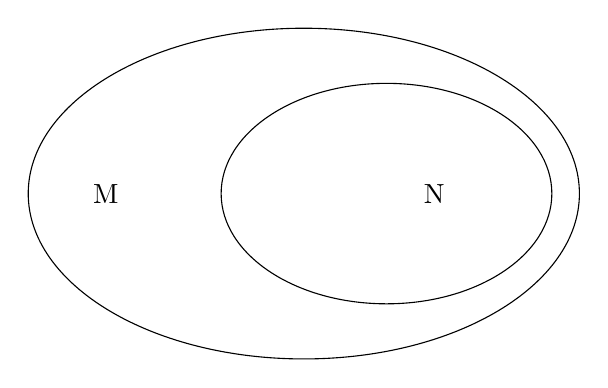
\begin{tikzpicture}[scale=0.7]
    \draw (0.0,0.0) ellipse (5.0 and 3.0);
    \draw (1.5,0.0) ellipse (3.0 and 2.0);
    \draw (-4.0,0.0) node[right]{M};
    \draw (2.0,0.0) node[right]{N};
  \end{tikzpicture}
  \caption{Teilmenge}
  \label{Abb:Mng:Teilmenge}
\end{center}
\end{figure}

Diese Abbildungen heißen 
\Begriff{Mengendiagramm}e oder auch \Begriff{Euler-Diagramm}e
\index[names]{Euler, Leonhard}\footnote{Leonhard Euler (1707-1783), 
schweizer Mathematiker,
\url{https://de.wikipedia.org/wiki/Leonhard_Euler}} oder 
\Begriff{Venn-Diagramm}e\index[names]{Venn, John}\footnote{John Venn
(1834-1923), englischer Logiker 
\url{https://de.wikipedia.org/wiki/John_Venn}}. Die 
Mengendiagramme dienen nur der Veranschaulichung! Sie können einem beim 
Beweisen als Anschauung helfen, sie ersetzen jedoch keinen Beweis!
\end{Unit}
\Translation{Mengendiagramm}{Venn diagram}

%% -----------------------------------------------------------------------------
\begin{Unit}[Bemerkung]
Aus der Definition der Gleichheit für Mengen und der Definition für Teilmengen 
ergibt sich

\begin{Bemerkung}
  Es seien $M$ und $N$ Mengen, dann gilt:
  \begin{align}
    (M = N) \Leftrightarrow (M \subseteq N) \wedge (N \subseteq M)\ .
  \end{align}
\end{Bemerkung}

Beweis: \newline
\begin{tabular}{l l l}
  & $M = N$ &\\
    $\Leftrightarrow$ & & (Definition der Gleichheit) \\
  & $\forall x : (x \in N) \leftrightarrow (x \in M)$ & \\
    $\Leftrightarrow$ & & (Aussagenlogik) \\
  & $\forall x : (x \in N) \rightarrow (x \in M)) \land$ & \\
  & $\forall x : (x \in M) \rightarrow (x \in N))$ & \\
    $\Leftrightarrow$ & & (Definition der Teilmenge) \\
  & $(N \subseteq M) \land (M \subseteq N)$ \ . & \\
\end{tabular}
 
\qed

Für den Beweis einer Mengengleichheit wird oftmals nachgewiesen, dass sich 
die beiden Mengen gegenseitig als Teilmengen enthalten.
\end{Unit}

%% -----------------------------------------------------------------------------
\begin{Unit}[Bemerkung]
Die Teilmengenbeziehung ist transitiv.
\begin{Bemerkung}
  Es seien $L$, $M$ und $N$ Mengen, dann gilt (Transitivität):
  \begin{align}
    (N \subseteq M) \wedge (M \subseteq L) \rightarrow\ (N \subseteq L)\ .
  \end{align}
  Ist $N$ eine Teilmenge von $M$ und $M$ eine Teilmenge von $L$, dann ist $N$ 
  auch eine Teilmenge von $L$.
\end{Bemerkung}

\begin{figure}[htbp]
\begin{center}
  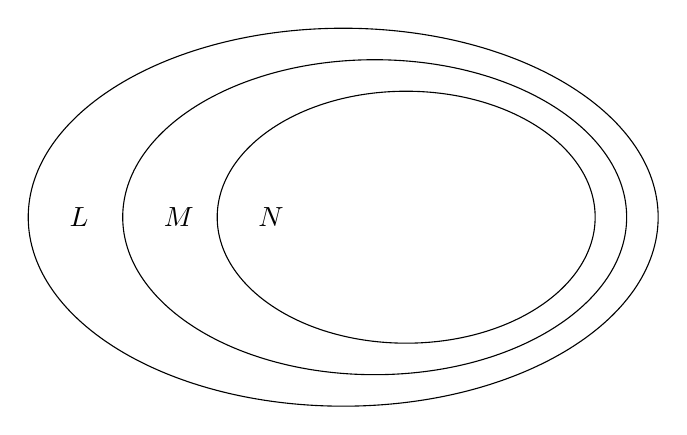
\begin{tikzpicture}[scale=0.8]
    \draw (0.0,0.0) ellipse (5.0 and 3.0);
    \draw (0.5,0.0) ellipse (4.0 and 2.5);
    \draw (1.0,0.0) ellipse (3.0 and 2.0);
    \draw (-4.5,0.0) node[right]{$L$};
    \draw (-3.0,0.0) node[right]{$M$};
    \draw (-1.5,0.0) node[right]{$N$};    
  \end{tikzpicture}
  \caption{Transitive Teilmengen}
  \label{Abb:Mng:Transitive Teilmengen}
\end{center}
\end{figure}

Beweis: Die Grafik (siehe Abbildung \ref{Abb:Mng:Transitive Teilmengen}) 
dient nur der Veranschaulichung. Der formale Beweis ist kurz. Für jedes 
$x \in N$ gilt:

\begin{tabular}{l l | l}
  & $(x \in N)$ &  \\
  $\Rightarrow$ & & $N$ ist Teilmenge von $M$ ($N \subseteq M$) \\
  & $(x \in M)$ & \\
  $\Rightarrow$ & & $M$ ist Teilmenge von $L$ ($M \subseteq L$) \\
  & $(x \in L)$ & \\
\end{tabular} 

\qed
\end{Unit}

%% -----------------------------------------------------------------------------
\begin{Unit}[Uebung]
Es seien $M\ =\ \{1, 2\}$ und $N\ =\ \{2, 3, 4\}$. Welche der folgenden 
Aussagen sind richtig?
\begin{itemize}
  \item $M \subseteq N$? \\
    Nein, da $1 \in M$, aber $1 \notin N$.
  \item $N \subseteq M$? \\
    Nein, da $4 \in N$, aber $4 \notin M$.
  \item $M\ =\ N$? \\
    Nein, da $4 \in N$, aber $4 \notin M$.
  \item $M\ \not=\ N$? \\
    Ja.
  \item $\{2, 4\}\ \subseteq N$? \\
    Ja.
  \item $2\ \in\ M$? \\
    Ja.
  \item $2\ \subseteq\ M$? \\
    Nein, dies ist nicht einmal ein gültiger Ausdruck, da $2$ keine Menge 
    ist, so dass keine Teilmengenbeziehung bestehen kann. Gültig wären die 
    Aussagen  $2\ \in\ M$ oder $\{2\} \subseteq\ M$.
  \item $\{2, \{3, 4\}\}\ \subseteq N$? \\
    Nein, die Menge auf der linken Seite besteht aus zwei Elementen, aus der 
    $2$ und aus der Menge mit den Elementen $3$ und $4$. Das zweite Element 
    ($\{3,4\}$) ist jedoch kein Element von $N$ (sondern eine Teilmenge von 
    $N$). Für die Teilmengenbeziehung müsste es jedoch Element von $N$ sein.
\end{itemize}
\end{Unit}

%% --- Potenzmenge -------------------------------------------------------------
%\subsection*{Potenzmenge}

%% -----------------------------------------------------------------------------
\begin{Unit}[Definition Potenzmenge]
Die Teilmengen einer Menge lassen sich selber wiederum zu einer Menge
zusammenfassen.

\begin{Definition}
Die Mengen aller Teilmengen einer Menge $M$ heißt \Begriff{Potenzmenge} von 
$M$: $\mathcal{P}(M)$.
\begin{align}
  \mathcal{P}(M) := \{T \mid T \subseteq M\}
\end{align}
\end{Definition}
\end{Unit}
\Translation{Potenzmenge}{power set}

%% -----------------------------------------------------------------------------
\begin{Unit}[Beispiel] \ 
\begin{enumerate}
  \item Es sei $M = \varnothing$, also die leere Menge, dann ist 
    $\mathcal{P}(M) = \{\varnothing\}$, also die Menge, die nur ein Element 
    hat, nämlich die leere Menge. Zu beachten ist, dass $\mathcal{P}(M)$ nicht 
    die leere Menge ist, sondern die Menge, die nur aus der leeren Menge 
    besteht!

  \item Es sei $M = \{a\}$ eine Menge, die aus einem Element besteht. Damit 
    ist die Potenzmenge die Menge, die aus der leeren Menge und der Menge 
    selbst besteht, denn das sind die einzigen Teilmengen der Menge $M$, also 
    $\mathcal{P}(M) = \{ \varnothing, M \}$.

  \item Es sei $M = \{a, b\}$ eine Menge mit genau zwei Elementen, dann ist 
    $\mathcal{P}(M) = \{ \varnothing, \{a\}, \{b\}, M \}$.
\end{enumerate}
\end{Unit}

%% -----------------------------------------------------------------------------
\begin{Unit}[Bemerkung]
Für endliche Mengen kann die Elementanzahl der Potenzmenge einfach angegeben
werden.

\begin{Bemerkung}
  Es sei $M$ eine endliche Menge mit $n = |M|$ Elementen, dann hat die 
  Potenzmenge von $M$ genau $2^n$ Elemente.
  \begin{align}
    ( |M| = n ) \rightarrow ( |\mathcal{P}(M)| = 2^n )
  \end{align}
\end{Bemerkung}

Der Beweis kann durch vollständige Induktion geführt werden, was hier jedoch 
nicht ausgeführt wird.
\end{Unit}

%% -----------------------------------------------------------------------------
\begin{Unit}[Bemerkung]
Eine Teilmengenbeziehung überträgt sich auch auf die Potenzmengen.

\begin{Bemerkung}
  Es seien $M$ und $N$ zwei beliebige Mengen. Ist $M$ eine Teilmenge von $N$, 
  dann ist die Potenzmenge von $M$ eine Teilmenge der Potenzmenge von $N$.
  \begin{align}
    M \subseteq N\ \rightarrow\ \mathcal{P}(M) \subseteq \mathcal{P}(N) 
  \end{align}
\end{Bemerkung}
Beweis: als Übung
\end{Unit}

%%------------------------------------------------------------------------------
%% Abschnitt: Operationen von Mengen
%%------------------------------------------------------------------------------
\section{Operationen von Mengen}
\label{sec:Mengen:Operationen von Mengen}

Wie kann mit Mengen gerechnet werden, welche Operationen gibt es und welche 
Regeln gibt es für die Operationen gibt.

%% --- Durchschnitt und Vereinigung --------------------------------------------
%\subsection*{Durchschnitt und Vereinigung}

%% -----------------------------------------------------------------------------
\begin{Unit}[Definition Durchschnitt]
Eine wichtige Verknüpfung von Mengen ist der Durchschnitt.

\begin{Definition}
  Es seien $M$ und $N$ beliebige Mengen. 
  Die Menge der Elemente, die sowohl in der Menge $M$, als auch in der Menge 
  $N$ sind, heißt der \Begriff{Durchschnitt} ($M \cap N$) von $M$ und $N$.
  \begin{align}
    M \cap N\ := \{ x \mid (x\in M) \land (x \in N) \}
  \end{align}
\end{Definition}
\Translation{Durchschnitt}{intersection}

\begin{figure}[htbp]
\begin{center}
  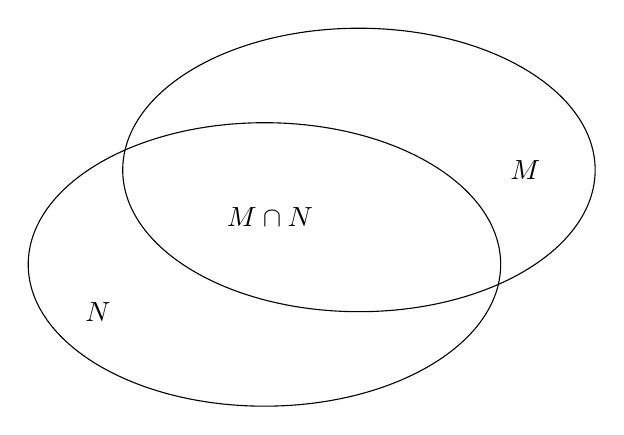
\begin{tikzpicture}[scale=0.6]
    \draw (0.0,0.0) ellipse (5.0 and 3.0);
    \draw (2.0,2.0) ellipse (5.0 and 3.0);
    \draw (-4.0,-1.0) node[right]{$N$};
    \draw (5.0,2.0) node[right]{$M$};
    \draw (-1.0,1.0) node[right]{$M \cap N$};
  \end{tikzpicture}
  \caption{Durchschnitt von Mengen}
  \label{Abb:Mng:Durchschnitt von Mengen}
\end{center}
\end{figure}

Die Abbildung (siehe \ref{Abb:Mng:Durchschnitt von Mengen}) veranschaulicht 
den Durchschnitt. Der Durchschnitt der Mengen $M$ und $N$ beinhaltet nur die 
kleine innere Fläche, die mit $M \cap N$ bezeichnet ist. 
\end{Unit}

%% -----------------------------------------------------------------------------
\begin{Unit}[Definition Vereinigung]
Eine weitere wichtige Verknüpfung von Mengen ist die Vereinigung.

\begin{Definition}
  Es seien $M$ und $N$ beliebige Mengen. 
  Die Menge der Elemente, die in der Menge $M$ oder in der Menge $N$ sind, 
  heißt die \Begriff{Vereinigung} ($M \cup N$) von $M$ und $N$.
  \begin{align}
    M \cup N := \{ x \mid (x \in M) \lor (x \in N) \}
  \end{align}
\end{Definition}
\Translation{Vereinigung}{union}
\end{Unit}

%% -----------------------------------------------------------------------------
\begin{Unit}[Definition disjunkt]
Die Eigenschaft, dass der Durchschnitt zweier Mengen die leere Menge ist, ist
eine besondere Eigenschaft.
 
\begin{Definition}
  Sind $M$ und $N$ zwei beliebige Mengen, mit leerem Durchschnitt ($M \cap N
  = \varnothing$), dann heißen $M$ und $N$ \Begriff{disjunkt}, und es wird 
  statt $M \cup N$ auch $M + N$ geschrieben.
\end{Definition}
\Translation{disjunkt}{disjoint}
\end{Unit}

%% --- Verallgemeinerter Durchschnitt und Vereinigung --------------------------
%\subsection*{Verallgemeinerter Durchschnitt und Vereinigung}

%% -----------------------------------------------------------------------------
\begin{Unit}[Anmerkung]
Durchschnitt und Vereinigung lassen sich nicht nur für zwei Mengen definieren. 
Ist $I$ eine beliebige (endliche oder unendliche) Indexmenge und ist jedem $i 
\in I$ eine Menge $M_i$ zugeordnet, so wird der \Begriff
{verallgemeinerten Durchschnitt} der Mengen $M_i$ mittels
\begin{align}
  \bigcap_{i \in I} M_i := \{ x \mid \forall i \in I: x \in M_i \} .
\end{align}
definiert.
Es ist die Menge der Elemente, die in jeder der Mengen $M_i$ enthalten ist.

Weiter wird definiert
\begin{align}
  \bigcup_{i \in I} M_i := \{x \mid \exists i \in I: x \in M_i \}
\end{align} die \Begriff{verallgemeinerte Vereinigung} der Mengen $M_i$. 
Es ist die Menge der Elemente, die in mindestens einer der Mengen $M_i$ 
enthalten ist.

Ist die Indexmenge gleich der leeren Menge, so ist der Durchschnitt die 
Grundmenge (!) und die Vereinigung die leere Menge (!), da die Bedingung 
$i \in I$ nicht erfüllt ist.
\end{Unit}

%% --- Assoziativ-, Kommutativ- und Distributivgesetz --------------------------
%\subsection*{Assoziativ-, Kommutativ- und Distributionsgesetz}

%% -----------------------------------------------------------------------------
\begin{Unit}[Satz]
Für das Rechnen mit Mengen gelten folgende Aussagen:

\begin{Satz}[Assoziativ-, Kommutativ- und Distributionsgesetz]
  Gegeben seien die Mengen $M$, $N$ und $L$ beliebige Mengen.
  Dann gelten die \Begriff{Assoziativgesetz}e
  \begin{align}
    M \cup (N \cup L) = (M \cup N) \cup L \\ 
    M \cap (N \cap L) = (M \cap N) \cap L\ ,
  \end{align}
  die \Begriff{Kommutativgesetz}e 
  \begin{align}
    M \cup N = N \cup M \\
    M \cap N = N \cap M
  \end{align}
  und die \Begriff{Distributivgesetz}e
  \begin{align}
    M \cup (N \cap L) = (M \cup N) \cap (M \cup L) \\
    M \cap (N \cup L) = (M \cap N) \cup (M \cap L) \ .
  \end{align}
\end{Satz}
\Translation{Assoziativgesetz}{associative law}
\Translation{Kommutativgesetz}{commutative law}
\Translation{Distributivgesetz}{distributive law}

Mit Hilfe der Mengendiagramme (siehe Abbildung \ref{Abb:Mng:Mengendiagramm}) 
lassen sich diese Sätze leicht veranschaulichen.

\begin{figure}[htbp]
\begin{center}
  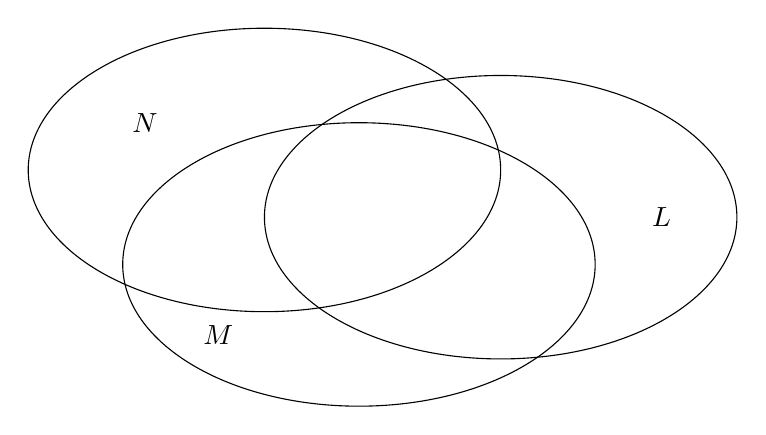
\begin{tikzpicture}[scale=0.6]
    \draw (0.0,0.0) ellipse (5.0 and 3.0);
    \draw (-2.0,2.0) ellipse (5.0 and 3.0);
    \draw (3.0,1.0) ellipse (5.0 and 3.0);
    \draw (-3.5,-1.5) node[right]{$M$};    
    \draw (-5.0,3.0) node[right]{$N$};
    \draw (6.0,1.0) node[right]{$L$};
  \end{tikzpicture}
  \caption{Mengendiagramm}
  \label{Abb:Mng:Mengendiagramm}
\end{center}
\end{figure}

Formal wird das Distributivgesetz bewiesen.

\begin{tabular}{l l | l}
    & $x \in M \cap (N \cup L)$ & \\
$\leftrightarrow$ & & (Definition Durchschnitt) \\
    & $(x\in M) \land (x \in (N \cup L))$ &  \\
$\leftrightarrow$ & & (Definition Vereinigung) \\
    & $(x\in M) \land ((x \in N) \lor (x\in L))$ & \\
$\leftrightarrow$ & & (Distributivgesetz - Aussagen) \\
    & $((x\in M) \land (x \in N)) \lor $ & \\
                  & $((x \in M) \land (x \in L))$ & \\
$\leftrightarrow$ & & (Definition Durchschnitt) \\
    & $(x \in M \cap N) \lor (x \in M \cap L)$ & \\
$\leftrightarrow$ & & (Definition Vereinigung) \\
    & $x \in (M \cap N) \cup (M \cap L)$ & \\
\end{tabular}

Somit wurde gezeigt, dass jedes Element $x \in M \cap (N \cup L)$ auch Element
von $(M \cap N) \cup (M \cap L)$, also $M \cap (N \cup L) \subseteq (M \cap N) 
\cup (M \cap L)$ und umgekehrt. Damit ist die beidseitige 
Teilmengenbeziehung gezeigt, und somit die Identität der beiden Mengen.\qed

Das Assoziativgesetz gilt nicht nur für drei Mengen, sondern auch für mehre 
Mengen. Daher kann hierbei auf die Klammersetzung verzichtet werden.
\end{Unit}

%% -----------------------------------------------------------------------------
\begin{Unit}[Bemerkung]
Für das Rechnen mit Mengen sind folgende Regeln oftmals nützlich:
\begin{Bemerkung}
  Es seien $M$ und $N$ beliebige Mengen, dann gelten
  \begin{align}
    M \cap (M \cup N) &= M \\
    M \cup (M \cap N) &= M \\
    M \cap M &= M \\
    M \cup M &= M
  \end{align}
\end{Bemerkung}
\end{Unit}

%% -----------------------------------------------------------------------------
\begin{Unit}[Bemerkung]
Für die leere Menge und die Grundmenge gelten folgende Aussagen:
\begin{Bemerkung}
  Es sei $M$ eine beliebige Teilmenge der Grundmenge $G$, dann gelten
  \begin{align}
    M \cap \varnothing &= \varnothing \\
    M \cup \varnothing &= M \\
    M \cap G &= M \\
    M \cup G &= G
  \end{align}
\end{Bemerkung}
\end{Unit}

%% --- Durchschnitt und Vereinigung bei Potenzmengen  --------------------------
%\subsection*{Durchschnitt und Vereinigung bei Potenzmengen}

%% -----------------------------------------------------------------------------
\begin{Unit}[Bemerkung]
Wie wirken sich der Durchschnitt und die Vereinigung von zwei Mengen auf die 
Potenzmengen aus, welchen Beziehungen gibt es?

\begin{Bemerkung}
  Es seien $M$ und $N$ zwei beliebige Mengen. Dann gelten \\
  (a) Die Potenzmenge des Durchschnitts der Mengen $M$ und $N$ ist gleich 
  dem Durchschnitt der Potenzmengen der Mengen $M$ und $N$.
  \begin{align}
    \mathcal{P}(M \cap N) = \mathcal{P}(M) \cap \mathcal{P}(N) 
  \end{align}
  (b) Die Vereinigung der Potenzmengen der Mengen $M$ und $N$ ist eine 
  Teilmenge der Potenzmenge der Vereinigung der Mengen $M$ und $N$.
  \begin{align}
    \mathcal{P}(M) \cup \mathcal{P}(N) \subseteq \mathcal{P}(M \cup N) 
  \end{align}
\end{Bemerkung}

Beweis: Übung. Bei (a) ist die gegenseitige Teilmengenbeziehung zu zeigen. 
Bei (b) ist nur die eine Richtung nachzuweisen. Wieso gilt die Gegenrichtung 
nicht? Finden Sie dazu ein Gegenbeispiel.
\end{Unit}

%% --- Durchschnitt und Vereinigung bei Potenzmengen  --------------------------
%\subsection*{Differenz und Komplement}

%% -----------------------------------------------------------------------------
\begin{Unit}[Definition Differenz, Komplement]
Im nachfolgenden seien $M$, $N$ und $L$ stets beliebige Mengen, die Teilmenge
einer festen Grundmenge $G$ sind.

\begin{Definition}
  (a) Es seien $M$ und $N$ beliebige Mengen, dann heißt
    \begin{align}
      M \backslash N := \{ x \mid (x \in M) \land (x \notin N) \} 
    \end{align}
    die \Begriff{Differenz} der Mengen $M$ und $N$. In der Differenz sind
    die Elemente von $M$, die nicht in $N$ sind. \\
  (b) Es sei $M$ eine beliebige Teilmenge von $G$, dann heißt die Menge
    \begin{align}
      \complement_G(M) := \{ x \in G \mid x \notin M \} = G \backslash  M
    \end{align}
    das \Begriff{Komplement} von $M$ bezüglich $G$. Es enthält die Elemente 
    der Grundmenge, die nicht in $M$ sind.
\end{Definition}
\Translation{Differenz}{difference}
\Translation{Komplement}{complementon}

Ist die Grundmenge $G$ allgemein bekannt, so kann das Komplement einer Menge 
$M$ kurz als $\overline{M}$ geschrieben werden. Durch die Umformulierung 
$\complement_G(M) := \{ x \in G \mid \neg(x \in M) \}$ wird der Zusammenhang 
zwischen Komplementbildung und der aussagenlogischen Negation deutlich.

Es ergibt sich sofort, dass $M$ und $\complement_G(M)$ disjunkt sind und dass 
$M + \complement_G(M) = G$ ist.
\end{Unit}

%% -----------------------------------------------------------------------------
\begin{Unit}[Bemerkung]
Wie wird die Differenzmenge mit Hilfe der Komplementmenge gebildet.

\begin{Bemerkung} 
  Es seien $M$ und $N$ beliebige Teilmengen einer Grundmenge $G$, dann gilt
  \begin{align}
    M \backslash N = M \cap \complement_G(N) \ .
  \end{align}
\end{Bemerkung}
Beweis: Übung
\end{Unit}

%% -----------------------------------------------------------------------------
\begin{Unit}[Definition symmetrische Differenz]
Wie wird die symmetrische Differenz mit Hilfe der Differenzen gebildet.

\begin{Definition}
  Es seien $M$ und $N$ Mengen, dann heißt
  \begin{align}
    M  \triangle N\ := (M \backslash N) + (N \backslash M) 
  \end{align}
  die \Begriff{symmetrische Differenz}\index{Differenz, symmetrische} 
  von $M$ und $N$.
\end{Definition}
\Translation{symmetrische Differenz}{symmetric difference}
Veranschaulichen Sie sich die Differenz.
\end{Unit}

%% -----------------------------------------------------------------------------
\begin{Unit}[Bemerkung]
Nochmals eine andere Möglichkeit, die symmetrische Differenz darzustellen.

\begin{Bemerkung} 
  Es seien $M$ und $N$ beliebige Teilmengen, dann gilt 
  \begin{align}
    M \triangle N = (M \cup N) \backslash (M \cap N) \ .
  \end{align}
\end{Bemerkung}
Beweis: Übung
\end{Unit}

%% --- Regeln von de Morgan ----------------------------------------------------
%\subsection*{Regeln von de Morgan}

%% -----------------------------------------------------------------------------
\begin{Unit}[Regel von de Morgan]
Wie bei den Aussagen gibt es auch hier Regeln von de Morgan.

\begin{Satz}
  Es seien $M$ und $N$ beliebige Teilmengen der Grundmenge $G$, dann gelten 
  die Sätze von de Morgan\index[names]{Morgan, Augustus de}\footnote{Augustus 
  de Morgan (1806-1871), englischer Mathematiker
(\url{https://de.wikipedia.org/wiki/Augustus_De_Morgan})} 
  \begin{align}
    \complement_G(M \cup N) &= \complement_G(M) \cap \complement_G(N) \\
    \complement_G(M \cap N) &= \complement_G(M) \cup \complement_G(N) \ .
  \end{align}
\end{Satz}

Ist die Grundmenge G bekannt, so wird kurz
\begin{align}
  \overline{(M \cup N)} &= \overline{M} \cap \overline{N} \text{ und } \\
  \overline{(M \cap N)} &= \overline{M} \cup \overline{N} 
\end{align}
geschrieben.

Beweis der ersten Aussage:\\
\begin{tabular}{l l | l}
                  & $x \in \complement_G(M \cup N)$ & \\
$\leftrightarrow$ & & (Definition Komplement) \\
                  & $(x \in G) \land (x \notin (M \cup N))$ & \\
$\leftrightarrow$ & & (Negation) \\
                  & $(x \in G) \land\neg (x \in (M \cup N))$ & \\
$\leftrightarrow$ & & (Definition Vereinigung) \\
                  & $(x \in G) \land$ & \\
                  &  $\neg((x \in M) \lor (x \in N))$ & \\
$\leftrightarrow$ & & (Satz von de Morgan - Aussagen) \\
                  & $(x \in G) \land $ &  \\
                  & $((\neg(x \in M)) \land (\neg(x \in N)))$ &  \\
$\leftrightarrow$ & & (Assoziativgesetz) \\
                  & $((x \in G) \land (\neg(x \in M)))$ & \\
                  & $\land ((x \in G) \land (\neg(x \in N)))$ & \\
$\leftrightarrow$ & & (Negation) \\
                  & $((x \in G) \land (x \notin M)) $ & \\
                  & $\land ((x \in G) \land (x \notin N)) $ & \\
$\leftrightarrow$ & & (Definition Komplement) \\
                  & $(x \in \complement_G(M) \land (x \in \complement_G(N))$ 
                    & \\
$\leftrightarrow$ & & (Definition Durchschnitt) \\
                  & $x \in \complement_G(M) \cap \complement_G(N)$ & \\
\end{tabular}

Auf Grund der Definition der Mengengleichheit gilt damit die behauptete 
Aussage. Der andere Teil kann analog bewiesen werden.
\qed
\end{Unit}

%% -----------------------------------------------------------------------------
\begin{Unit}[Anmerkung]
Auch für Familien von Mengen gelten die verallgemeinerter Sätze von de Morgan
\index[names]{Morgan, Augustus de}.
\begin{align}
  \complement_G(\bigcap_{i \in I}M_i) = \bigcup_{i \in I}\complement_G(M_i) \\
  \complement_G(\bigcup_{i \in I}M_i) = \bigcap_{i \in I}\complement_G(M_i)
\end{align}
\end{Unit}
%%------------------------------------------------------------------------------

%%------------------------------------------------------------------------------
%% Abschnitt: Klasseneinteilung
%%------------------------------------------------------------------------------
\section{Klasseneinteilung}
\label{sec:Mengen:Klasseneinteilung}

%% -----------------------------------------------------------------------------
\begin{Unit}[Definition Klasseneinteilung]
Im folgenden sei $I$ stets eine beliebige Indexmenge.

\begin{Definition}
  Es sei $\{M_i \mid i \in I)\}$ eine Familie von beliebigen nicht leeren 
  Teilmengen einer Grundmenge. Die Familie von Mengen heißt 
  \textbf{(paarweise) disjunkt}\index{disjunkt, paarweise}, wenn für alle 
  $i, j \in I$ die Mengen $M_i$ und $M_j$ disjunkt sind: 
  \begin{align}
    \{ M_i \mid i \in I \} \text{ paarweise disjunkt} :\Leftrightarrow\
      \forall i,j \in I, i \not= j: M_i \cap M_j = \varnothing \ .
  \end{align} 
  Eine Familie von Mengen heißt \Begriff{Klasseneinteilung} oder 
  \Begriff{disjunkte Zerlegung}\index{Zerlegung, disjunkte} oder 
  \Begriff{Partition} von $G$, wenn sie paarweise disjunkt ist und die 
  verallgemeinerte Vereinigung der Mengen gleich der Grundmenge ist.
\end{Definition}
\Translation{paarweise disjunkt}{pairwise disjoint}
\Translation{Klasseneinteilung}{partition}
\Translation{Zerlegung}{partition}

\begin{figure}[htbp]
\begin{center}
  \begin{tikzpicture}
    \draw (0,0) -- (0,4) -- (8,4) -- (8,0) -- (0,0);
    \draw (2,0) -- (2,4);
    \draw (4,0) -- (4,4);
    \draw (6,0) -- (6,4);
    \draw (2,2) -- (6,2);
    \draw (0,2) node[right]{$M_1$};    
    \draw (2,3) node[right]{$M_2$};
    \draw (2,1) node[right]{$M_3$};
    \draw (4,3) node[right]{$M_4$};
    \draw (4,1) node[right]{$M_5$};
    \draw (6,2) node[right]{$M_6$};
  \end{tikzpicture}
  \caption{Klasseneinteilung}
  \label{Abb:Mng:Klasseneinteilungn}
\end{center}
\end{figure}

Klasseneinteilungen treten an vielen Stellen auf. In Abbildung 
\ref{Abb:Mng:Klasseneinteilungn} ist eine Klasseneinteilung dargestellt:
paarweise disjunkt, die Vereinigung ist die komplette Grundmenge.
\end{Unit}

%% -----------------------------------------------------------------------------
\begin{Unit}[Beispiel]
  Die natürlichen Zahlen lassen sich in die disjunkten Mengen der geraden und 
  der ungeraden Zahlen zerlegen.
\end{Unit}

%% -----------------------------------------------------------------------------
\begin{Unit}[Beispiel]
  Ist $P$ die Menge der Produktion der Automobile eines Werkes an einem Tag. 
  Es werden die verschiedenen Baumuster $B_1,\ldots, B_n$ produziert und 
  seien $T_1, \ldots, T_n$ die Menge der Autos der Tagesproduktion mit diesen 
  Baumustern, dann ist $\{T_i\ ;\ i = 1,\ldots,n\}$ die Klasseneinteilung der 
  Tagesproduktion $P$.
\end{Unit}

%% -----------------------------------------------------------------------------
\begin{Unit}[Definition Äquivalenzklassen]
Durch die Klasseneinteilung einer Menge $G$ ist jedes Element von $G$ genau 
in einer Teilmenge der Klasseneinteilung enthalten.

\begin{Definition}
  Sind zwei Elemente $x$, $y$ in der gleichen Teilmenge einer 
  Klasseneinteilung, so heißen sie \Begriff{äquivalent} ($x \sim y$). Die 
  Teilmengen der Klasseneinteilung heißen auch \Begriff{Äquivalenzklassen}. 
  Ein Element einer Äquivalenzklasse heißt \Begriff{Repräsentant} der
  Äquivalenzklasse.
\end{Definition}
\end{Unit}
\Translation{äquivalent}{equivalent}
\Translation{Äquivalenzklasse}{equivalence class}
\Translation{Repräsentant}{representative}

%% -----------------------------------------------------------------------------
\begin{Unit}[Bemerkung]
Für Äquivalenzklassen gibt es einige Eigenschaften, die bei der Behandlung 
von Relationen noch genauer betrachtet werden.
 
\begin{Bemerkung}
  Es seien $x$, $y$ und $z$ Elemente aus einer Menge $G$ mit einer 
  Klasseneinteilung. Für die Äquivalenz $\sim$ der Klasseneinteilung 
  gelten: \\
  (a) Für jedes $x \in G$ ist $x \sim x$, das heißt, dass die 
    Klasseneinteilung \Begriff{reflexiv} ist. \\
  (b) Ist $x \sim y$, sind also $x$ und $y$ in derselben Äquivalenzklasse, 
    dann gilt auch $y \sim x$, das heißt, dass die Klasseneinteilung 
    \Begriff{symmetrisch} ist. \\
  (c) Ist $x \sim y$ und $y \sim z$, dann ist auch $x \sim z$, das heißt, 
    dass die Klasseneinteilung \Begriff{transitiv} ist.
\end{Bemerkung}
\end{Unit}
\Translation{reflexiv}{reflexive}
\Translation{symmetrisch}{symmetric}
\Translation{transitiv}{transitive}

%% -----------------------------------------------------------------------------
\begin{Unit}[Beispiel]
  Die Menge der ganzen Zahlen $\ZZ$ wird bezüglich des Rests bei der Division 
  durch $6$ in sechs verschiedene Äquivalenzklassen aufgeteilt. Für 
  $i = 0, 1, 2, 3, 4, 5$ seien $T_i$ die Menge der ganzen Zahlen, die bei der
  Division durch $6$ den Rest $i$ haben. 
  \begin{align}
    T_i = \{x \in \ZZ \mid \exists n \in \ZZ : x = 6n + i \}
  \end{align}
  Dies definiert eine Klasseneinteilung: $\ZZ = T_0 + T_1 + T_2 + T_3 + T_4 + 
    T_5$. \\
  Für einen Repräsentanten und jeden Vertreter einer der Klassen $T_2$, $T_4$ 
  oder $T_6$ gilt, dass er durch zwei teilbar ist. Die Repräsentanten der 
  Klassen $T_3$ und $T_6$ sind jeweils durch 3 teilbar. Daher können in den 
  Klassen $T_2$, $T_3$, $T_4$ und $T_6$ keine Primzahlen enthalten sein 
  (Ausnahme: $2$ und $3$ selbst). Durch die gemeinsame Eigenschaft der Zahlen 
  der Klassen kann dies für jedes Element der Klasse bewiesen werden.
\end{Unit}

%% -----------------------------------------------------------------------------
\begin{Unit}[Anmerkung]
Ist $n$ eine beliebige natürliche Zahl, so kann die Menge $\ZZ$ in $n$ 
disjunkte Teilmengen bezüglich der Division durch $n$ zerlegt werden. Die 
Teilmengen $T_i$ für $i = 0, 1, \ldots, n-1$, werden folgendermaßen gebildet: 
\begin{align}
  T_i := \{ x \in \ZZ \mid \exists k \in \ZZ: x = kn+i \}
\end{align}
Diese Teilmengen bilden eine Klasseneinteilung der ganzen Zahlen. Die Menge 
$\ZZ_n = \{0, 1, \ldots, n-1\}$ bildet ein Repräsentantensystem. Dieses 
Repräsentantensystem wird im Folgenden noch vorkommen. Es hat eine wichtige
Bedeutung in der Informatik.
\end{Unit}

%% -----------------------------------------------------------------------------
\begin{Unit}[Anmerkung]
Die Klassenaufteilung ist ein häufig verwendetes Verfahren, um die 
Problemlösung oder andere Aufgaben auf eine begrenzte Zahl von Fällen zu 
reduzieren. Bei Meinungsumfragen werden die Befragten in bestimmte Klassen
eingeteilt, um dann Aussagen über die Vertreter dieser Klassen im allgemeinen 
zu erhalten.

Auch die Fallunterscheidungen ist eine Klasseneinteilung. Auch 
Fallunterscheidungen kommen an vielen Stellen vor, zum Beispiel bei der 
Definition von mathematischen Funktionen, bei der Berechnung der privaten 
Steuerlast, in Programmvorgaben, um nur einige wenige Beispiele  zu nennen.
\end{Unit}

%%------------------------------------------------------------------------------

%%------------------------------------------------------------------------------
%% Abschnitt: Kartesisches Produkt
%%------------------------------------------------------------------------------
\section{Kartesisches Produkt}
\label{sec:Mengen:Kartesisches Produkt}

%% -----------------------------------------------------------------------------
\begin{Unit}[Anmerkung]
In vielen Fällen ist es sinnvoll, geordnete Paare $(x, y)$ von Elementen $x \in 
X$ und $y \in Y$ zweier Mengen $X$ und $Y$ zu betrachten. Dabei heißt $x$ die
erste Komponente und $y$ die zweite Komponente. Ein Beispiel hierfür ist das 
2-dimensionale Koordinatensytem, bei dem $X = \RR$ und $Y = \RR$ gilt. Die 
Gleichheit zweier geordneter Paare wird durch
\begin{align}
  (x_1,y_1) = (x_2,y_2) :\Leftrightarrow (x_1 = x_2) \land (y_1 = y_2)
\end{align}
definiert. Die Mengen $X$ und $Y$ können jedoch auch beliebige Mengen sein.
\end{Unit}

%% -----------------------------------------------------------------------------
\begin{Unit}[Definition Kartesisches Produkt für zwei Mengen]
Zuerst die Definition eines kartesischen Produktes bei zwei Mengen. 

\begin{Definition}
  Es seien $X$ und $Y$ zwei beliebige Mengen, dann heißt die Menge
  \begin{align}
    X \times Y := \{ (x,y) \mid x \in X \land y \in Y \} \ ,
  \end{align}
  also die Menge der geordneten Paare $(x,y)$ mit $x \in X$ und $y \in Y$ das
  \Begriff{kartesische Produkt} der Mengen $X$ und $Y$. Die Elemente 
  dieses kartesischen Produktes heißen auch \Begriff{geordnete 2-Tupel}
  \index{Tupel, geordnetes 2-}.
\end{Definition}
\Translation{kartesisches Produkt}{Cartesian product}
\Translation{Tupel}{tuple}

Das kartesische Produkt ist nach Ren\`{e} Descartes\footnote{Ren\`{e} 
Descartes (1596-1650) französischer Philosoph und Mathematiker,
\url{https://de.wikipedia.org/wiki/Ren\%C3\%A9_Descartes}} 
\index[names]{Descartes, Ren\`{e}} benannt. Das kartesische Produkt ist 
selber wieder eine Menge, deren Elemente die geordneten 2-Tupel sind.
\end{Unit}

%% -----------------------------------------------------------------------------
\begin{Unit}[Beispiel]
In der Regel ist $X \times Y$ ungleich $Y \times X$. Die Gleichheit ist
hier die Mengengleichheit. Diese Aussage kann anhand des ersten Beispiel
sofort gesehen werden.

  Es seien $X = \{1, 2, 3\}$ und $Y = \{a, b\}$, dann ist
  \begin{align}
    X \times Y = \{ (1,a), (1,b), (2,a), (2,b), (3,a), (3,b) \}
  \end{align}
  und
  \begin{align}
    Y \times X = \{ (a,1), (a,2), (a,3), (b,1), (b,2), (b,3) \} \ .
  \end{align}
  Die beiden kartesischen Produkte sind ungleich.
\end{Unit}

%% -----------------------------------------------------------------------------
\begin{Unit}[Beispiel]
  Es seien $P = \{ p_1, p_2, p_3, p_4 \}$ eine Menge von Produkten und $L = 
  \{ l_1, l_2, l_3 \}$ eine Menge von Lieferanten. Dann ist $P \times L$ das 
  kartesische Produkt der Produkte und Lieferanten.
\end{Unit}

%% -----------------------------------------------------------------------------
\begin{Unit}[Beispiel]
  Es seien $X = Y = \NN$, dann ist $\NN \times \NN$ die Menge der geordneten 
  Paare von natürlichen Zahlen.
\end{Unit}

%% -----------------------------------------------------------------------------
\begin{Unit}[Beispiel]
  Es seien $X = Y = \RR$, dann ist $\RR \times \RR$ die Menge der geordneten 
  Paare von reellen Zahlen, der zweidimensionale Anschauungsraum.
\end{Unit}

%% -----------------------------------------------------------------------------
\begin{Unit}[Definition Kartesisches Produkt]
Die Definition des kartesischen Produktes kann verallgemeinert werden. Das 
Produkt kann auch für drei oder mehr Mengen gebildet werden.

\begin{Definition}
  Es sei $n \in \NN$ und $X_i$ ($i = 1, \ldots, n$) beliebige nicht leere 
  Mengen. Dann heißt die Menge
  \begin{align}
    \prod_{i=1}^n X_i := \{ (x_1, x_2, \ldots, x_n) \mid \forall_{i=1}^n x_i 
      \in X_i \} \ ,
  \end{align}
  die Menge aller (geordneten) $n$-Tupel $(x_1, x_2, \ldots, x_n)$ mit $x_i 
  \in X_i$ für alle $i \in \{1, 2, \ldots, n\}$, das \Begriff{kartesische 
  Produkt} von $X_1, X_2, \ldots , X_n$.
\end{Definition}

Statt $\prod_{i=1}^n X_i$ wird auch $X_1 \times X_2 \times \cdots \times 
X_n$ geschrieben. Die Definition kann auch auf Folgen von Mengen 
$\{ X_n \}_{n \in \NN}$ verallgemeinert werden.

Ist $n = 2$, so heißt $X_1 \times X_2$ auch \Begriff{Paarmenge}. Für 
$n = 1$ ist das kartesische Produkt gleich der Menge $X_1$. Sind $X_1 = X_2 = 
\cdots = X_n = X$, so wird für $\prod_{i=1}^n X_i$ auch kurz $X^n$ geschrieben. 
Beispiele für spezielle kartesische Produkte sind $\RR^2$ und $\RR^3$, die zwei- 
und dreidimensionalen Anschuungsräume.
\end{Unit}

%% -----------------------------------------------------------------------------
\begin{Unit}[Bemerkung]
Bei einem (endlichen) kartesisches Produkt von endlichen Mengen, kann die
Elementanzahl des kartesischen Produktes berechnet werden.

\begin{Bemerkung}
  Es seien für $n \in \mg{N}$ die Mengen $X_1, X_2, \ldots , X_n$ endlich mit 
  den Elementanzahlen $|X_i| = m_i$. Dann gilt $|\prod_{i=1}^n X_i| = 
  \prod_{i=1}^n m_i $.
\end{Bemerkung}
\end{Unit}
